\begin{algorithmic}
  \State $x \coloneqq x$
\end{algorithmic}

\begin{center}
  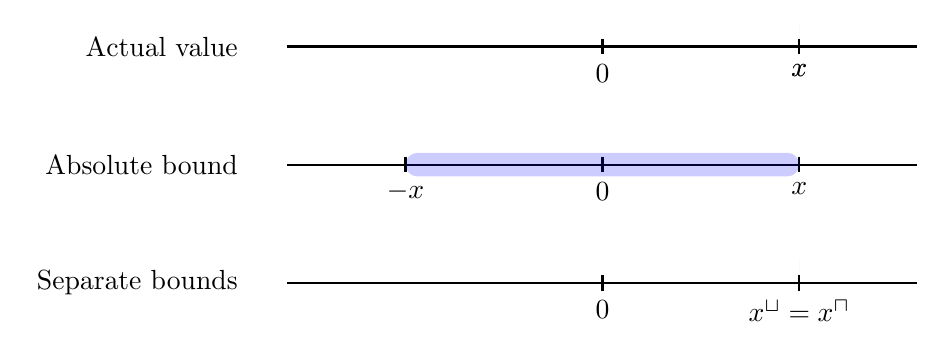
\begin{tikzpicture}[scale=0.5]
    \foreach \i/\y/\lvalue/\uvalue/\llabel/\ulabel/\name in {
      2/6/5/5/$x$/$x$/\text{Actual value},
      3/3/-5/5/$-\abs{x}$/$\abs{x}$/\text{Absolute bound},
      4/0/5/5/$x^\sqcup=x^\sqcap$/\text{}/\text{Separate bounds}
    } {
      \onslide<\i->{
        \draw[-, thick] (-8,\y) node[left=0.5cm] {\name} -- (8,\y);
        \draw[thick] (0,\y+0.2) -- (0,\y-0.2) node[below] {0};
        \draw[thick] (\lvalue,\y+0.2) -- (\lvalue,\y-0.2) node[below] {\llabel};
        \draw[thick] (\uvalue,\y+0.2) -- (\uvalue,\y-0.2) node[below] {\ulabel};
        \fill[opacity=0.2,blue,rounded corners=1ex] (\lvalue,\y-0.3) -- (\uvalue,\y-0.3) -- (\uvalue,\y+0.3) -- (\lvalue,\y+0.3) -- cycle;
      }
    }
  \end{tikzpicture}
\end{center}
